\subsection{Descriptions}
The common-drain amplifier shown in Figure 1 is constructed, using two $10k$\si{\ohm} resistors in parallel for the $5k$\si{\ohm} resistor.
These resistors are measured to have a parallel resistance of $4.924k$\si{\ohm}.

\FloatBarrier

\begin{figure}[h!]
	\centering
	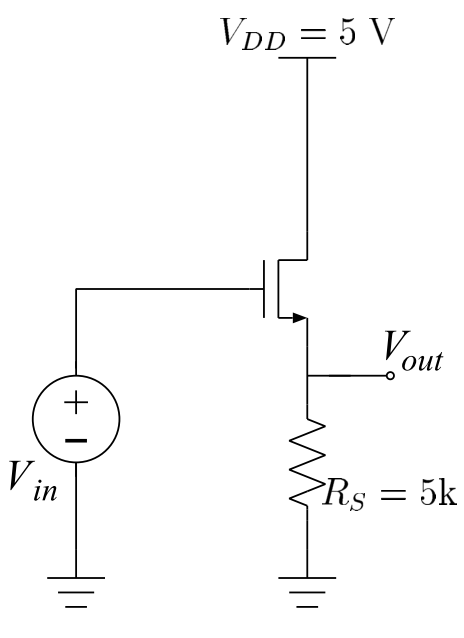
\includegraphics[scale=0.45]{./images/circuit_1.PNG}
	\caption{Common-Drain Amplifier}
	\label{fig:circuit_1}
\end{figure}

\FloatBarrier

With $V_{DS}$ constant at $5$\si{\volt}, $V_{GS}$ is swept from 0 to $5$\si{\volt} to obtain the voltage transfer characteristic shown in Figure (\ref{fig:part1_vtc}) and Table (\ref{tab:part1_vtc}).

Next, a $10$\si{\milli\volt} signal is applied to $V_{in}$, starting off at $1$\si{\kilo\hertz} under the assumption that the amplifier performs better when at lower frequencies. The amplifier should have a higher low-frequency gain because of the transistor's parasitics, such as the junction capacitances between the doped regions. At higher frequencies, these parasitic capacitances dominate, causing the FET to act like a low-pass filter, thereby decreasing the high-frequency gain.
The frequency is subsequently increased to $100$\si{\kilo\hertz} and then $1$\si{\mega\hertz}. Oscilloscope screenshots are shown for each frequency in Figures (\ref{fig:SCOPE_0}), (\ref{fig:SCOPE_2}), and (\ref{fig:SCOPE_3}), respectively.
The gains at each frequency are tabulated in Table (\ref{tab:gain_part1}).

This procedure is repeated when biasing the transistor $10$\si{\milli\volt} higher. Results are shown in Figures (\ref{fig:SCOPE_6}), (\ref{fig:SCOPE_5}), and (\ref{fig:SCOPE_4}), respectively, and gains are tabulated in Table (\ref{tab:gain_part1_plus10mV}).

\subsection{Calculation}

\FloatBarrier

\begin{table}[h!]
	\centering
	\caption{Figure (\ref{fig:part1_vtc}) Data}
	\label{tab:part1_vtc}
	\csvautotabular{./tables/part1_vtc.csv}
\end{table}

\FloatBarrier

\begin{table}[h!]
	\centering
	\caption{Figure (\ref{fig:SCOPE_4}) Data}
	\label{tab:gain_part1_plus10mV}
	\csvautotabular{./tables/gain_part1_plus10mV.csv}
\end{table}

\FloatBarrier

\begin{table}[h!]
	\centering
	\caption{Figure (\ref{fig:SCOPE_3}) Data}
	\label{tab:gain_part1}
	\csvautotabular{./tables/gain_part1.csv}
\end{table}

\FloatBarrier

For this circuit, $V_{out} = I_{D}R_{S}$, so $V_{out} = 0$\si{\volt} while the transistor is in cutoff. Afterward, even when Vin = $5$\si{\volt}, $V_{DS}$ is more than $V_{in} - V_{t}$ so that the transistor is in saturation any time it is on.
The threshold voltage appears to be around $1.4$\si{\volt}.
For maximum possible input swing, the circuit is biased at the middle of the saturation region where $V_{in} = V_{in(eq1)} = 3.3$\si{\volt}.
$3.3$\si{\volt} is acquired by finding the midpoint of $V_{out}$ and then determining the $V_{in}$ for which that $V_{out}$ occurs.
Here, the midpoint of $V_{out}$ occurs at $\frac{2.65 + 0.00}{2} \approx 1.33$\si{\volt}.
This occurs when $V_{in} \approx 3.3$\si{\volt}.
Thus, $V_{in(eq1)} \approx 3.3$\si{\volt}.

\subsection{Analysis}

\FloatBarrier

\begin{figure}[h!]
	\centering
	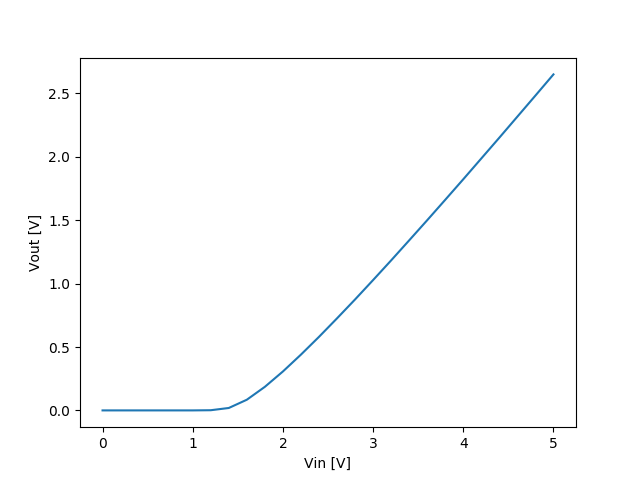
\includegraphics[scale=0.45]{./images/part1_vtc.PNG}
	\caption{$V_{out}$ vs $V_{in}$ for the Common-Drain Amplifier}
	\label{fig:part1_vtc}
\end{figure}

\FloatBarrier

\FloatBarrier

\begin{figure}[h!]
	\centering
	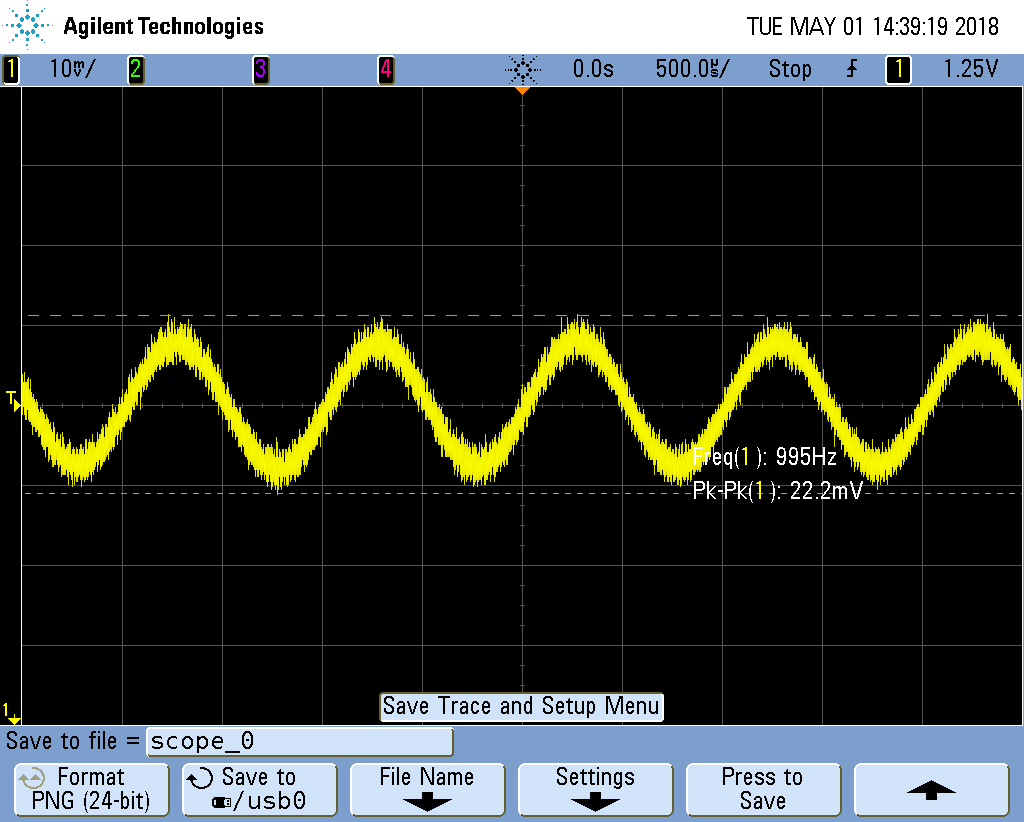
\includegraphics[scale=0.45]{./images/SCOPE_0.PNG}
	\caption{Amplified Waveform of a $1$\si{\kilo\hertz} Signal of Peak-to-Peak Amplitude of $20$\si{\milli\volt}}
	\label{fig:SCOPE_0}
\end{figure}

\FloatBarrier

\begin{figure}[h!]
	\centering
	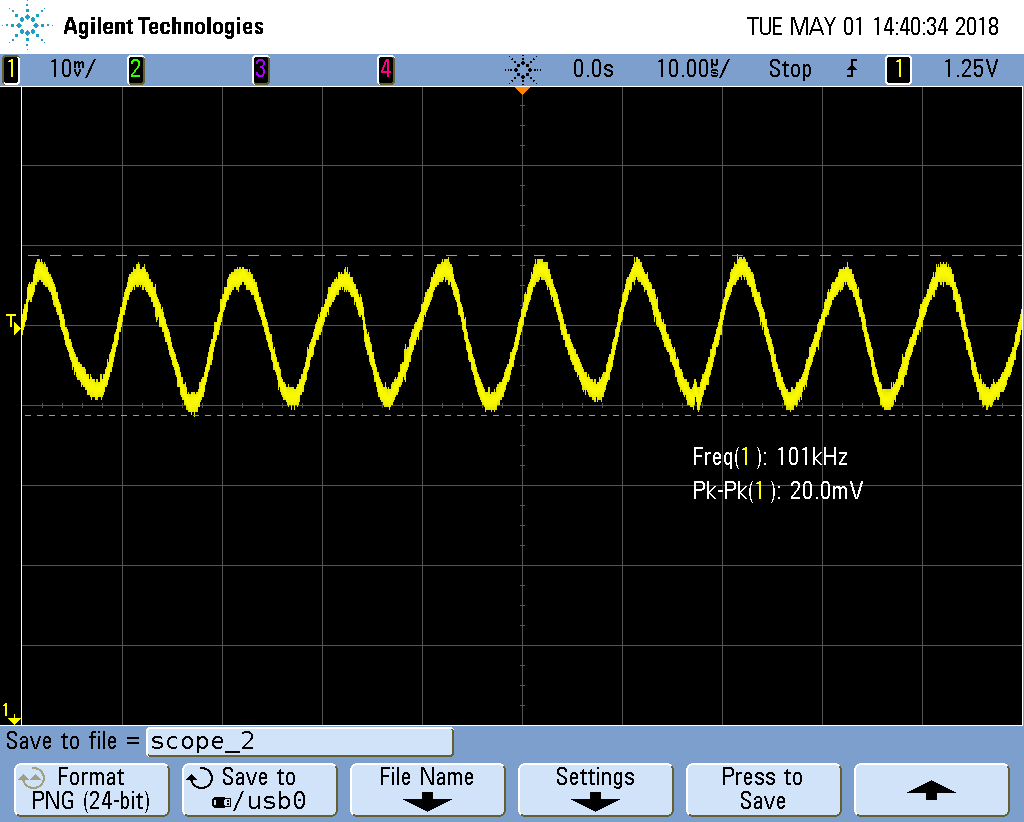
\includegraphics[scale=0.45]{./images/SCOPE_2.PNG}
	\caption{Amplified Waveform of a $100$\si{\kilo\hertz} Signal of Peak-to-Peak Amplitude of $20$\si{\milli\volt}}
	\label{fig:SCOPE_2}
\end{figure}

\FloatBarrier

\begin{figure}[h!]
	\centering
	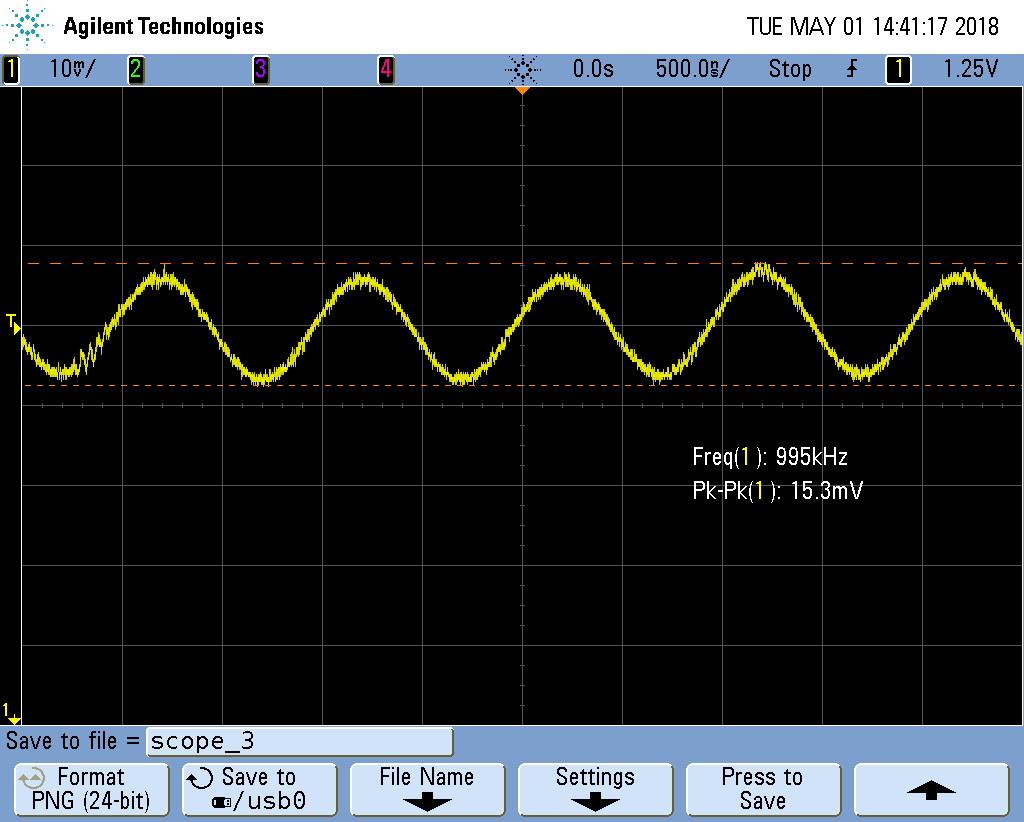
\includegraphics[scale=0.45]{./images/SCOPE_3.PNG}
	\caption{Amplified Waveform of a $1$\si{\mega\hertz} Signal of Peak-to-Peak Amplitude of $20$\si{\milli\volt}}
	\label{fig:SCOPE_3}
\end{figure}

\FloatBarrier

The varying gains as a function of frequency shows that the amplifier is not as effective at higher frequencies. In order for this circuit to function as a voltage follower or buffer as it is intended, the signal frequency should stay near $100$\si{\kilo\hertz}.

\FloatBarrier

\begin{figure}[h!]
	\centering
	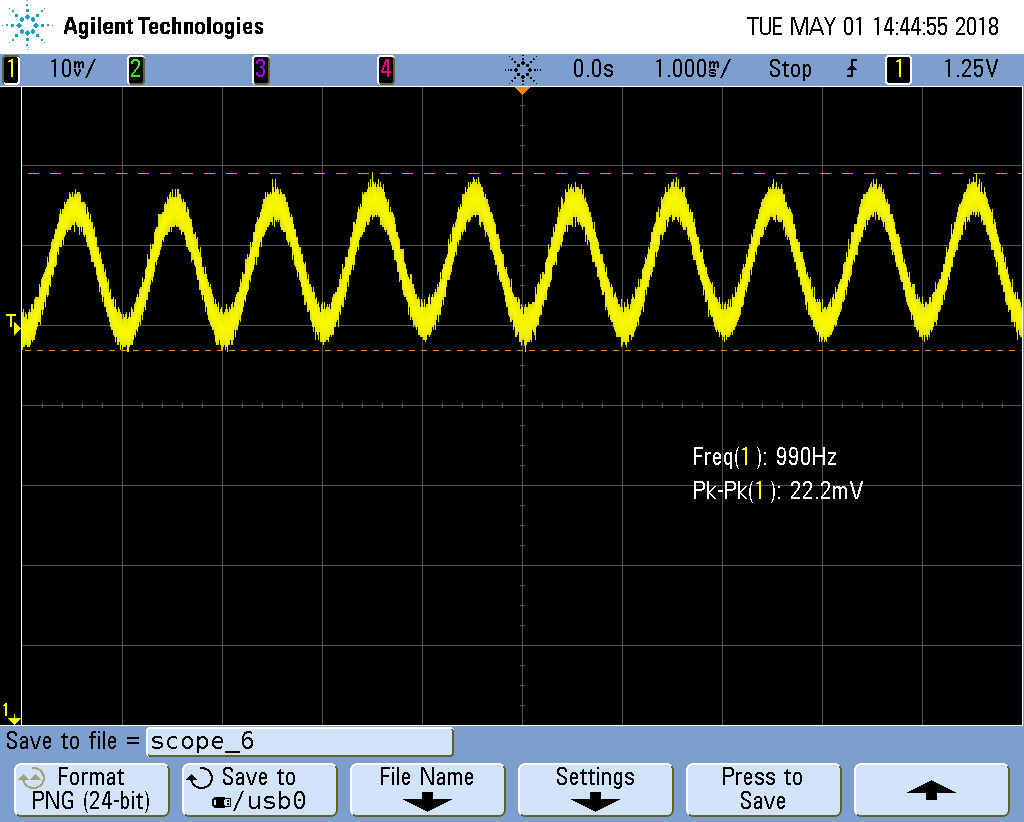
\includegraphics[scale=0.45]{./images/SCOPE_6.PNG}
	\caption{Amplified Waveform of a $1$\si{\kilo\hertz} Signal of Peak-to-Peak Amplitude of $20$\si{\milli\volt}}
	\label{fig:SCOPE_6}
\end{figure}

\FloatBarrier

\begin{figure}[h!]
	\centering
	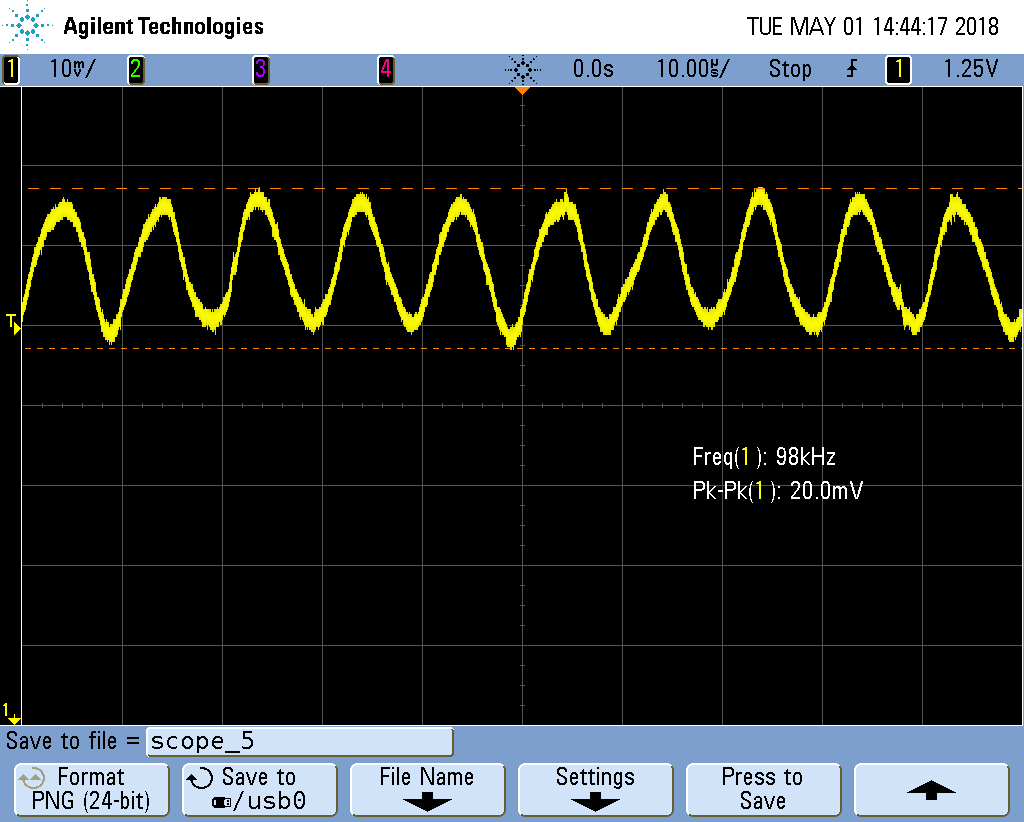
\includegraphics[scale=0.45]{./images/SCOPE_5.PNG}
	\caption{Amplified Waveform of a $100$\si{\kilo\hertz} Signal of Peak-to-Peak Amplitude of $20$\si{\milli\volt}}
	\label{fig:SCOPE_5}
\end{figure}

\FloatBarrier

\begin{figure}[h!]
	\centering
	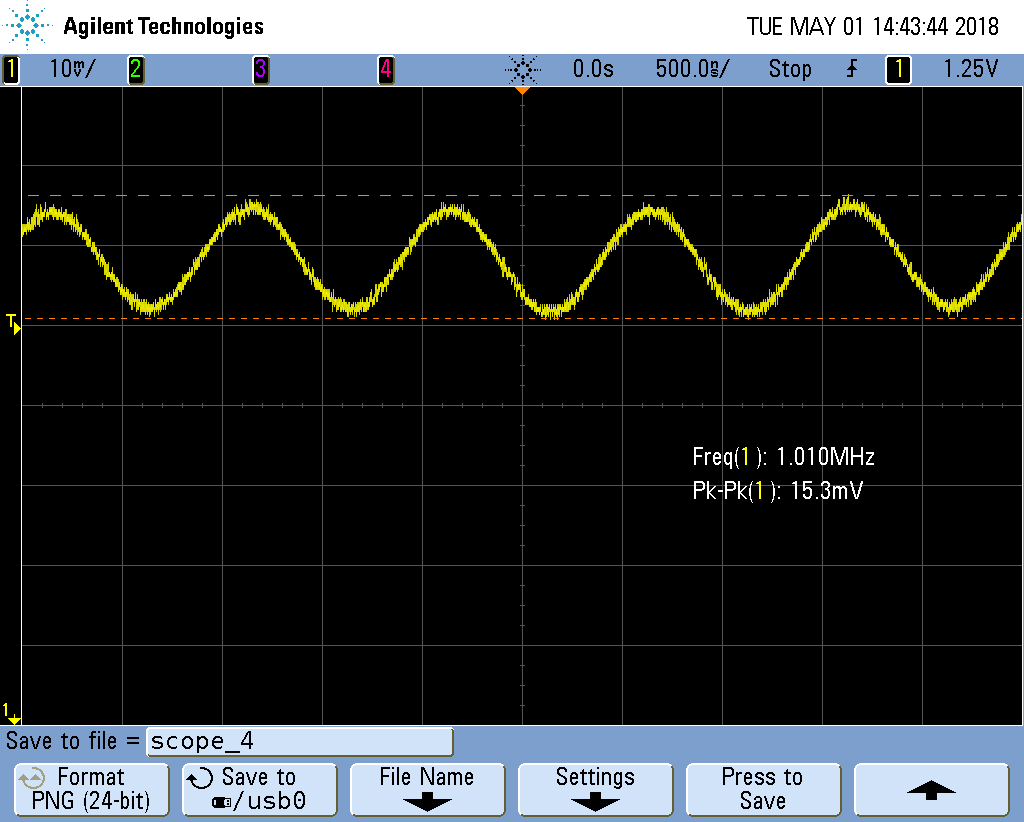
\includegraphics[scale=0.45]{./images/SCOPE_4.PNG}
	\caption{Amplified Waveform of a $1$\si{\mega\hertz} Signal of Peak-to-Peak Amplitude of $20$\si{\milli\volt}}
	\label{fig:SCOPE_4}
\end{figure}

\FloatBarrier

Due to the nearly uniform slope of the VTC in the saturation region, the gain as a function of the bias voltage is nearly constant.
Thus, these waveforms and gains are practically identical to what is observed earlier.
